\chapter{Deep Reinforcement Learning for Traffic Signal Control along Arterials}
\label{chap:arterial}

% !TEX root = main.tex
\section{Method}

In this section, we first present our context-aware RL design and then we discuss how to transfer knowledge between agents for more efficient learning.

\subsection{Model framework: DRL agent with context}
\label{sec:agent-design}

Our individual RL agent follows the state-of-the-art RL framework on a single intersection, namely $\Deeplight$~\cite{wei2018intellilight}. The most significant difference is in the state and reward design, where we add context features on approaching and receiving lanes into state representation to realize coordination and use queue length in reward design.

\paragraph{Design of agent.}We specify the design of three components in RL:

\begin{itemize}[wide,noitemsep,topsep=0pt]
\item \textbf{State.}  Three kinds of features are included in our state: current phase $\phase$ and the total number of vehicles $\numOfVehicles_\laneIndex$ on approaching lane $i$ which are included in \cite{wei2018intellilight}, and a feature about contextual information - the distribution of vehicles $\distriOfVehicles_\laneIndex$ on approaching lanes. Without losing generality, in this paper, each lane $\laneIndex$ is equally binned into $K$ segments by their relative position to the center of the intersection. Then $\distriOfVehicles$ is a tuple $<\distriOfVehicles_{\laneIndex,1},\dots, \distriOfVehicles_{\laneIndex,K}>$ with each element calculated by the number of vehicles on each segment. $k= 1$ indicates the farthest segment to the intersection and $k = K$ indicates the closest segment to the intersection. 
In this paper, we have $K=3$, where each lane is binned into 3 segments. We prove that more than two segments would be efficient to describe the context, detailed in Section~\ref{sec:app-proof}. 

\begin{figure*}[t!]
  \centering
   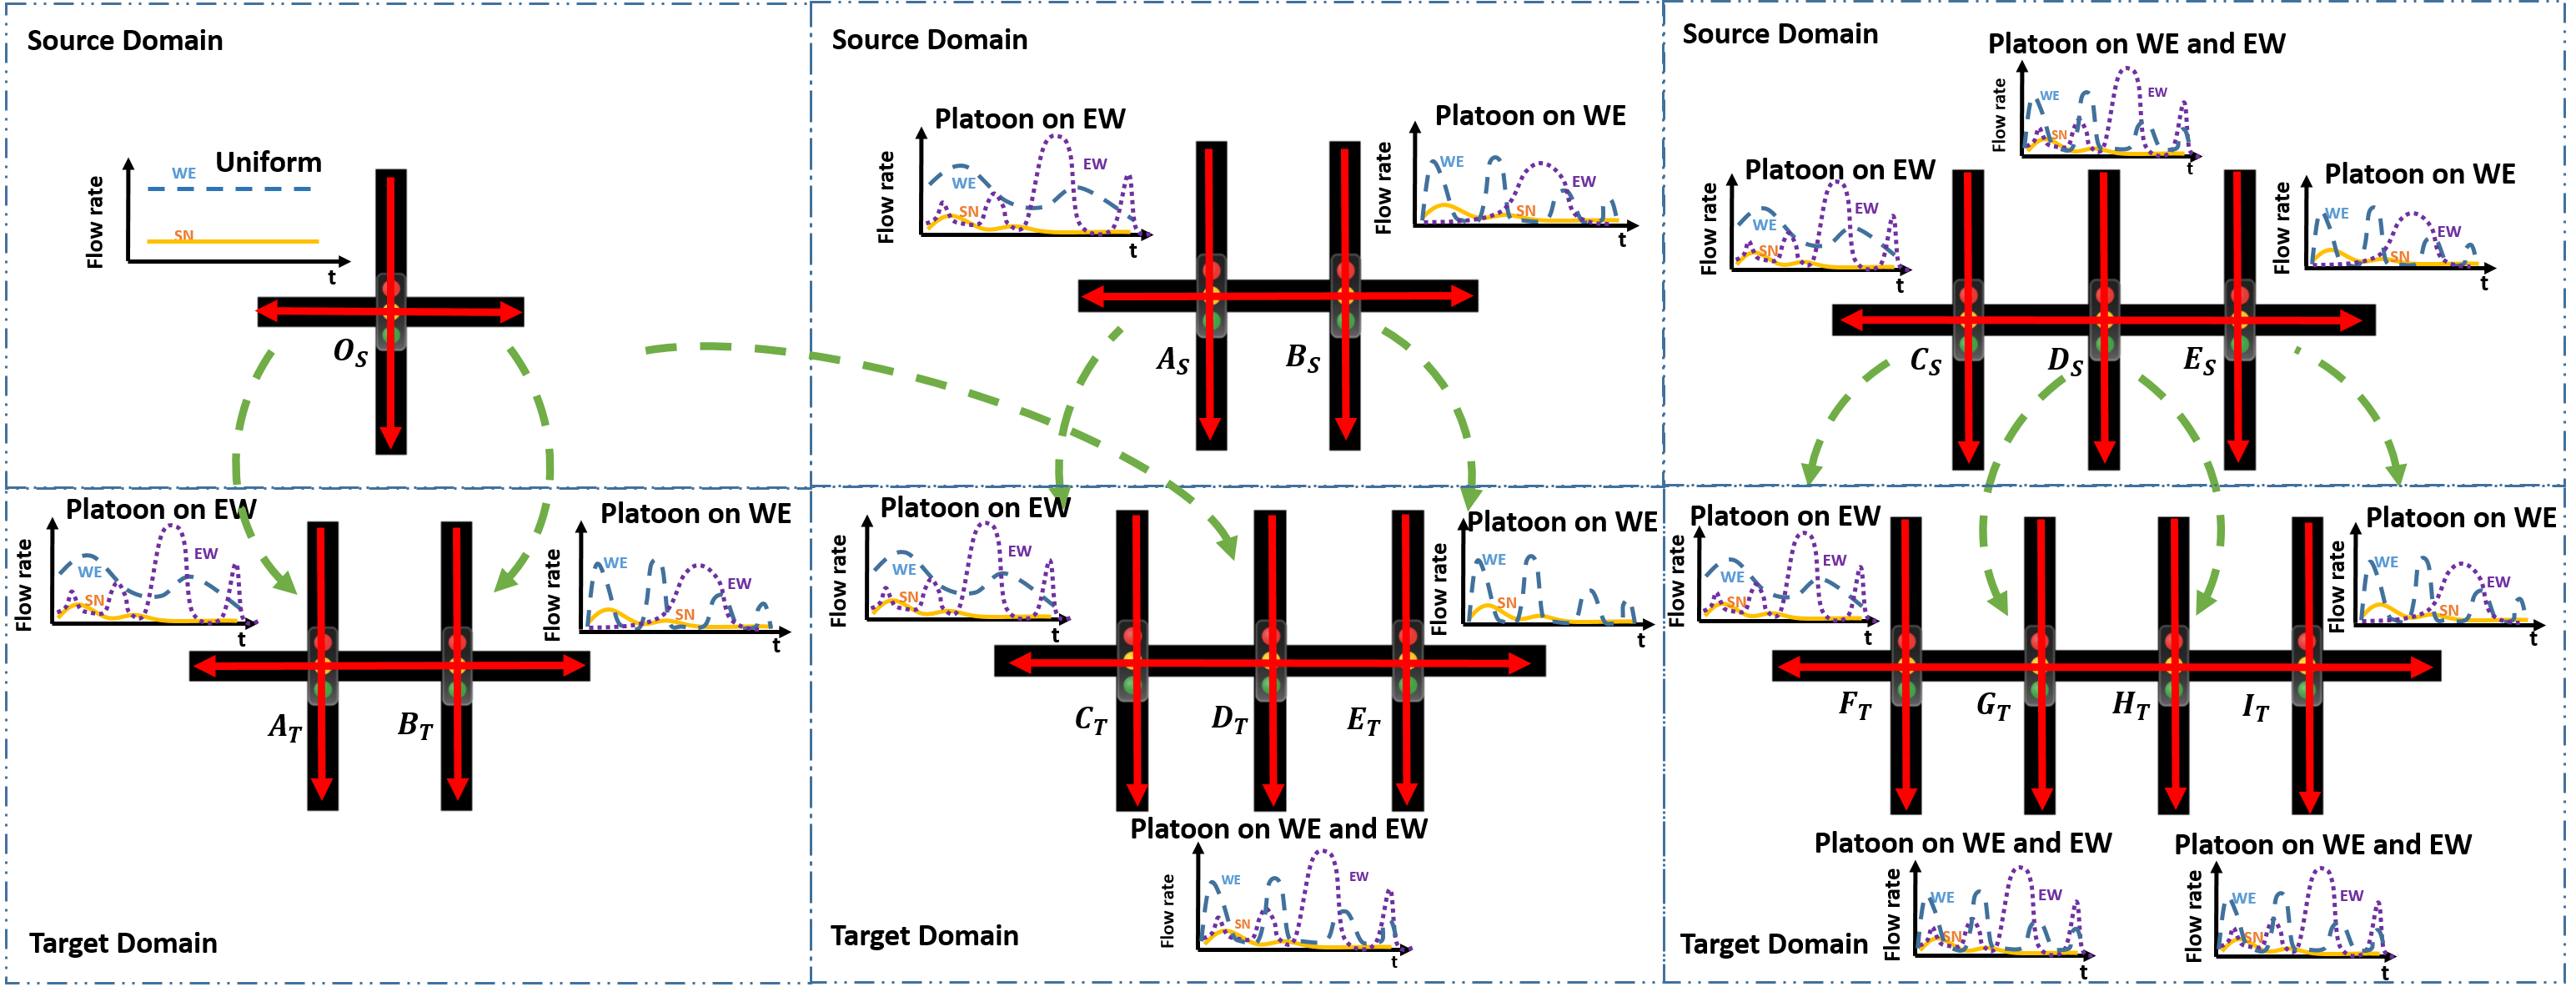
\includegraphics[width=0.95\textwidth]{figures/transfer3.pdf}
    \caption{Transfer RL agents for multi-intersection from existing knowledge to new network. Similar agents in traffic flow network can be transferred. Left to right: Transfer from isolated intersection to a  2-intersection corridor, from 2-intersection to 3-intersection corridor, from 3-intersection to 4-intersection corridor.}
   \label{fig:transfer}
\end{figure*}


\item \textbf{Action.} The action is defined as $\action=1$: change the light to next phase, and $\action = 0$: keep the current phase.


\item \textbf{Reward.} Our reward is defined as a sum of queue length $\queueLength$ over all approaching lanes, where
$\queueLength$ is calculated as the total number of waiting vehicles on the given lane. A vehicle with a speed of less than 0.1 m/s is considered waiting.
\end{itemize}

\paragraph{Justification of state and reward design.}
In existing literature~\cite{VaOl16,liLW16,GenR16,wei2018intellilight}, the state includes various kinds of features, including current phase, number of vehicles on road, delay, queue length, duration, image representation of vehicle position, etc. However, none of them theoretically justify which ones are useful. Intuitively, coordinating the traffic signals along an arterial mainly includes two decisions: a) phase split and b) offset. In our state definition, queue length helps decision (a), and the context information helps decision (b). Intuition suggests the information is sufficient for the traffic signal coordination. Going beyond intuition, we can also prove that the features we used in state definition are capable of describing the environment for an individual RL agent to learn a cooperation strategy.

Coordinating the traffic signals along arterial tries to minimize the average travel time (or equivalently delay) of vehicles under uniform traffic. We can prove that by setting reward as queue length, optimizing the reward individually is equal to optimizing the global average travel time. Due to the page limit, the proof of the proposed state and reward design is included in the cover letter.


\subsection{Learning Process}
In this paper, we adopt similar network structure as~\cite{wei2018intellilight} for Deep Q-Network (DQN) to estimate the Q-value function as $Q(s, a; \theta)$, as shown in Figure~\ref{fig:q-network}.  Features are concatenated and fed into fully-connected layers. Then, phase gate is used to activate different branch of the network: when phase $\phase = 1$, the upper branch will be activated; when phase $\phase = 0$, the lower branch will be activated. This will distinguish the decision process for different phases, prevent the decision from favoring specific action, and enhance the fitting ability of the network.
%In this paper, we adopt similar network structure as~\cite{wei2018intellilight} for Deep Q-Network (DQN) to estimate the Q-value function as $Q(s, a; \theta)$. 
Periodically, the agent will take samples from memory and use them to update the network as is stated in Equation~\ref{eq:loss},  where a sample is a tuple of $<s,a,r,s'>$, $s$, $a$ and $r$ are the current state, action and corresponding reward, $s'$ is the next state, and  $i$ stands for the $i$-th iteration.
\begin{equation}
\label{eq:loss}
\mathcal{L}_i(\theta_i) = \mathbb{E}_{s,a,r,s'}[r+\gamma\max_{a'}Q(s',a';\theta_{i-1})-Q(s,a;\theta_{i-1})^2]
\end{equation}

\begin{figure}[h!]
  \centering
   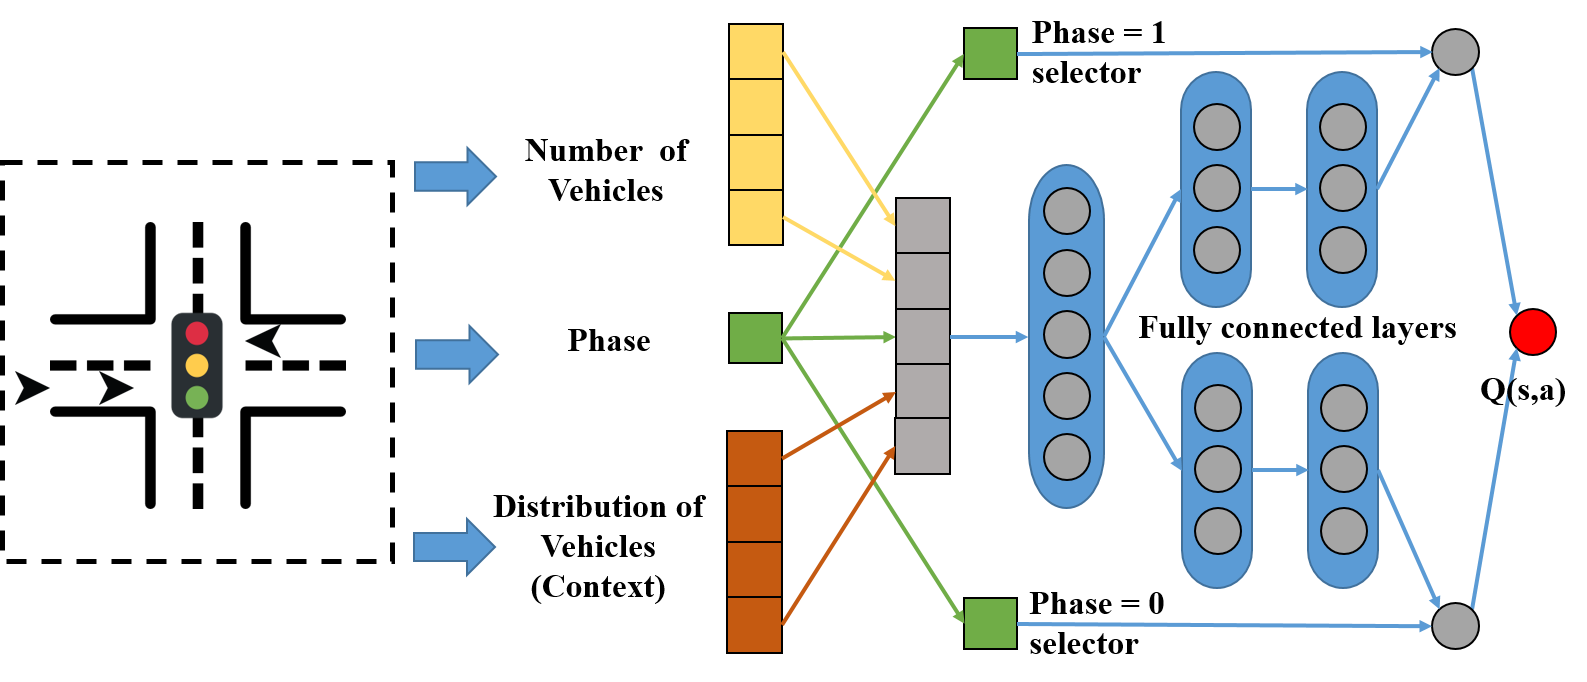
\includegraphics[width=0.45\textwidth]{figures/network1.png}
    \caption{Q-Network structure}
   \label{fig:q-network}
\end{figure}

\subsection{Transferring RL agents}
In this section, we briefly introduce the process of transferring RL agents for traffic signal control problem. If we train each RL agent from scratch, the computational cost is high. Therefore, we propose to transfer knowledge, i.e., the Q-value function, between agents for a quicker convergence and better performance. 

% Transfer learning~\cite{taylor2009transfer} of RL often use value functions from a set of source tasks as an initialization for a related target task, which is then refined by further learning. Therefore, we use the value functions of smaller source tasks as heuristics for the larger target task. Although there are no theoretical guarantees that these Q-functions are appropriate for the new problem, transfer planning is more efficient due to its decoupling of a large, multi-agent problem into smaller source problems that can be solved more easily.

We formalize the transfer problem as follows: Given the set of RL tasks $\Sigma=\{\sigma\}$, the set of agents $\pmb{G}^\sigma$ for task $\sigma$, and the mapping from each Q-value component $Q$ to a task $M(Q)=\sigma\in\Sigma$, the transfer problem for multi-intersection signal control is to find a mapping $\mathcal{P}$ from source task $\sigma_S$ to target task $\sigma_T$. We only have to define the source tasks, the corresponding mapping $\mathcal{P}_{\sigma_T}$ for each target task $\sigma_T$, and find a heuristic Q-value function $Q_{\sigma_S}$ for each mapped source task.

In traffic signal control scenario, first, the agents $\pmb{G}$ for simple scenarios (isolated agent or two agents) in Figure~\ref{fig:transfer} are trained. Then the Q-value functions from $\pmb{G}$ are re-used as the value functions $Q_{\sigma_S}$ from source tasks. The corresponding mapping $\mathcal{P}_{\sigma_T}$ is simply defined by the similarity of each agent based on the topology of the traffic network. 

Figure~\ref{fig:transfer} shows the pipeline of transferring RL agents with bidirectional traffic on the arterial. In this process, the Q-value function is transferred. Firstly we need to train a basic RL for isolated control task $O_S$ and then re-use it for target tasks in 2-intersection arterial ($A_T, B_T$). After the target task is learned, we can 
transfer from the 2-intersection corridor to a 3-intersection corridor ($C_T, D_T, E_T$), with $D_T$  transferred from $O_S$, $C_T$ and $E_T$ transferred from $A_S$ and $B_S$ since their traffic flow changes similarly (e.g., both $C_T$ and $E_T$ have platoon traffic on \WE). Similarly, after 3-intersection corridor ($C_S, D_S, E_S$) is learned, they can be re-used correspondingly to a 4-intersection corridor ($F_T, G_T, H_T, I_T$). For intersections with complex structure, transferred RL agents serves as an initialization.


%The reason why we design $\mathcal{P}$ in this way is straightforward. Since $Q$ is the action-value function for policy $\pi:\mathcal{S}\times\mathcal{A}\rightarrow[0,1]$, it is a mapping from the traffic condition and action tuple to the expected reward. Since the target and source agents that are similar in the traffic flow network, their learned policy $\pi$ could also be similar. 





\nop{
Deploying pipeline framework not only make the model converge faster but also serves as a guarantee to converge. As it is mentioned above, the behavior of the neighboring agents significantly affects whether or not the agent could learn a good policy. If the upstream agent behaves randomly, for instance, it could cast a bad influence on the downstream agent. Hence, the basic idea of pipeline pre-training is to alleviate the bad influence of neighboring agents in the learning process of the specific agent.


Nonetheless, to train each agent in a sequential manner could be a huge cost even it is in the process of pre-training. Hence, the idea of transfer learning is further exploited to help agents learn faster with the use of learned knowledge by similar intersection agents. For now, the similarity of each agents is defined by the topology of the network. In the future, a traffic pattern detection module may be applied to measure the similarity to intelligently.


transfer learning instead of multi-agent reinforcement learning is that the non-stationarity that appears when multiple agents learn in tandem is circumvented. Moreover, by learning the Q-function to a much simpler problem and then re-using it, less time has to be spent training. If the factors in the graph are very similar, only a single source problem needs to be found, which can be re-used for every factor.


Before the training process of corridor intersections, several single-intersection agents are learned with basic traffic configurations, e.g., uniform or platoon traffic flow and their combinations on different directions. Once the Q-value function for the single-intersection scenario is learned, this is used as the source problem in transfer learning.  To solve the multi-intersection scenarios, this source problem is used for each agents. 

However, if the distribution of samples from source domain is far more different with target domain, it is critical to select the suitable source domain to be transferred. For corridor intersections, the intersections receiving traffic on a corridor is different from \Todo{} \todo{ba zhongwen xie xialai...}. 

Whichever kind of traffic looks, the traffic will seem to looks like platoon after passing the start and end of corridor.\todo{chacha: did you write this??} Therefore, we train the single agent for uniform traffic firstly, then transfer pretrained agent to first and last intersections, then train the agents together with other intersections. (how can we select similar traffic files?)
For the first intersection, we train the RL using isolated traffic 
}



% !TEX root = main.tex
\section{Experiment}



\subsection{Experimental Setup}
We configure our experimental setup using on SUMO (Simulation of Urban Mobility)~\footnote{\url{http://sumo.dlr.de/index.html}}, an open-source microscopic simulation package with flexible settings in network design, traffic simulation and traffic light control.

\paragraph{Road network setting.}We use both synthetic and real-world road networks to define the network in the simulator. A single intersection, unless otherwise specified, is set to be a four-way intersection, with four 300-meter long road segments and six lanes with opposite directions of travel. Hence each intersection has three incoming and three outgoing lanes for each direction. The maximum speed on the road segments is set to 40 kilometers/hour. Vehicles can always turn right when there is no conflicting traffic. Every time the phase switches, a 5-second combined yellow and all-red time are followed to clear the intersection.


\begin{figure*}[t!]
  \centering
  \begin{tabular}{cc}
   \includegraphics[width=0.48\textwidth]{figures/case_beaver.png} &
   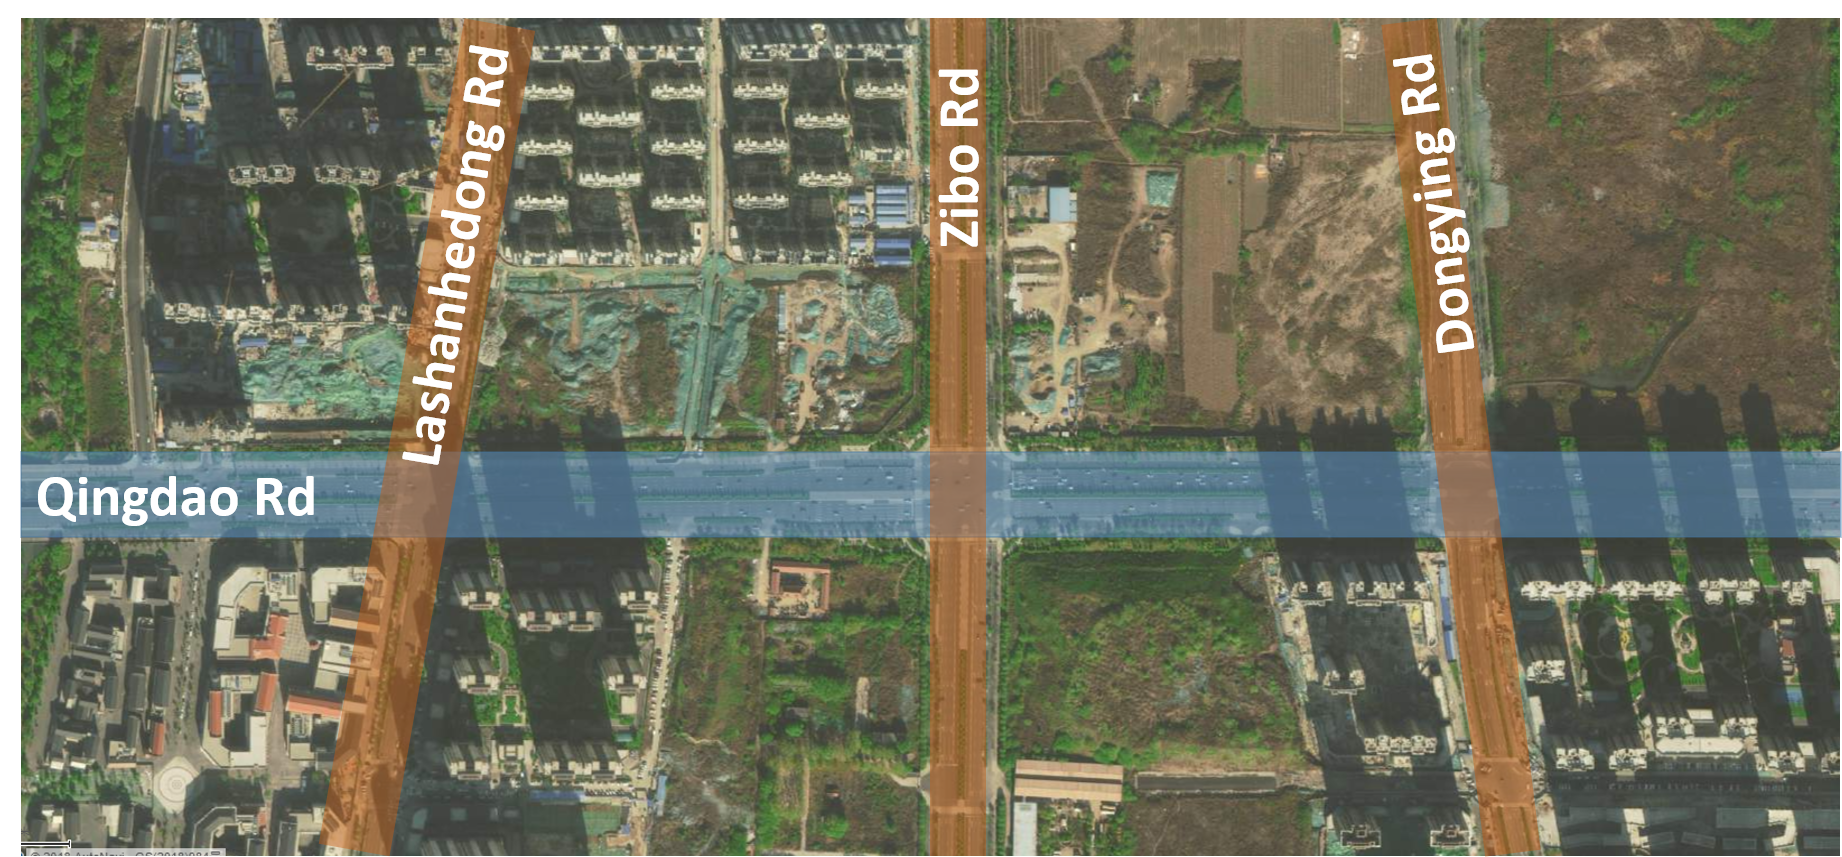
\includegraphics[width=0.38\textwidth]{figures/case_intersection_note.png} \\
   \begin{tabular}[c]{@{}c@{}}(a) Beaver Avenue in State College, Pennsylvania, USA: \\a 5-intersection arterial with unidirectional traffic on the arterial\\ and bidirectional traffic on the side streets.\end{tabular}&
   \begin{tabular}[c]{@{}c@{}}(b) Qingdao Road in Jinan, China:\\ a 3-intersection arterial with bidirectional traffic \\on both the arterial and the side streets.\end{tabular}\\
   \end{tabular}
   
     \caption{Real-world arterials for experiment.}
    \label{fig:real-intersection}
\end{figure*}


\paragraph{Evaluation metric.}Following existing studies, we use the average \textit{travel time} to evaluate the performance (other measures show similar performance and are not shown here due to space limit), which calculates average travel time the vehicles spent within the system (in seconds). This is the most frequently used measure for traffic signal performance in the transportation field.

\paragraph{Compared methods.}We compare our model with the following methods, whose detailed configuration can be found in the cover letter. It should be noted that all methods are carefully tuned and their best results are reported~\footnote{The codes including parameter settings are available at authors' website}. 

\begin{itemize}[wide,noitemsep,topsep=0pt]

\item \textbf{\FT}: Fixed-time with random offset~\cite{Roess2011t}. The offsets are randomly selected to mimic an arterial without any coordination.

\item \textbf{\Greenwave}~\cite{Roess2011t} is a closed-form solution under uniform one-way traffic, providing green waves for one direction on the arterial. 
This is the most classical method in transportation field to implement coordination. However, \Greenwave is only optimal in terms of average travel time for uniform one-way traffic on the arterial. 

\item \textbf{\Maxband}~\cite{little1981maxband} provides the green wave for two directions on the arterial. 

\item \textbf{\NIPS}~\cite{VaOl16} is a coordinated reinforcement learning approach for multi-intersection control by designing a coordination graph and learning the joint local Q-function for two adjacent intersections.


\item \textbf{\Deeplight}~\cite{wei2018intellilight} is an individual deep reinforcement learning approach. This method does not consider context information. %  \Deeplight is a single intersection control model that uses a representation of the local traffic information as state and reward function.

\end{itemize}

We denote our proposed method as \textbf{\MTDeeplight}. Our proposed method without transfer learning is denoted as \textbf{\MDeeplight}.  


\paragraph{Traffic flow dataset.}
Both synthetic and real-world traffic flow datasets are utilized in the experiment. Each vehicle in the traffic flow dataset is described as $(o,t,d)$, where $o$ is origin location, $t$ is time, and $d$ is destination location. Locations $o$ and $d$ are both locations on the road network. Traffic data is taken as input for the simulator. A detailed description of the datasets is included in the cover letter.
\begin{itemize}[wide,noitemsep,topsep=0pt]

\item Synthetic traffic:  Uniform traffic with turning movements is utilized as synthetic traffic with two different arrival rates on the arterial: 300 vehicles/hour/lane (light traffic) and 500 vehicles/hour/lane (heavy traffic). The arrival rates on the side streets are 30\% of the arterial. All the vehicles on approaching lanes will have 20\% of possibility to turn left and 20\% turning right.

\item Real-world traffic: We collect two representative traffic flow data through manually counting and roadside cameras for two cities: Beaver Avenue in State College, USA, and Qingdao Road in Jinan, China. Figure~\ref{fig:real-intersection} shows the aerial view on these arterials.
\end{itemize}


\begin{center}
\begin{table}[h!]
\vspace{-3mm}
\caption{Performance of adopted methods w.r.t average travel time on a 4-intersection arterial. Lower the better. }
\label{tab:overall-result}
\begin{tabular}{ccccc}
\toprule
     & \begin{tabular}[c]{@{}c@{}}Synthetic\\ light\end{tabular} & \begin{tabular}[c]{@{}c@{}}Synthetic\\ heavy\end{tabular} & \begin{tabular}[c]{@{}c@{}}State\\ College\end{tabular}& Jinan \\ \hline \midrule
\multicolumn{5}{c}{Transportation baselines}                                                                                                   \\ \hline
\FT   & 77.51                                                     & 91.93                                                     & 58.63  & 159.20 \\
\Greenwave   & 67.26                                                     & 67.20                                                     & 48.56  & 140.71 \\
\Maxband   & 71.20                                                     & 65.93                                                     & -*      & 97.97  \\
\hline
\multicolumn{5}{c}{RL baselines}                                                                                                               \\ \hline
\NIPS  & 67.59                                                     & 84.87                                                     & 37.28  & 97.66  \\
\Deeplight  & 65.28                                                     & 68.68                                                     & 38.29  & 95.86  \\
\hline
\multicolumn{5}{c}{Ours}                                                                                                                       \\ \hline
\MDeeplight  & 64.79                                                     & 65.36                                                     & 37.01  & 89.23  \\
\MTDeeplight & \textbf{64.78}**                                                     & \textbf{65.34}**                                                    & \textbf{36.30}**  & \textbf{86.25}**  \\
\bottomrule
\end{tabular}
\\\footnotesize{${*}$ \Maxband is not applicable on the one-way arterial.}
\\\footnotesize{${**}$ denotes a significance with p-value $< 0.05$ over the second best model (except our variant) based on a two-tailed paired t-test.}
\end{table}
\end{center}

\vspace{-3mm}
\subsection{Experiment Results}

\subsubsection{Overall performance}

Table~\ref{tab:overall-result} shows the average travel time performance on synthetic and real-world data. 
We have the following observations:

1) Our proposed method \MTDeeplight achieves the best performance compared with state-of-the-arts, including the methods with explicit coordination strategies (\Greenwave, \Maxband and \NIPS). This demonstrates that, even without explicit coordination, our RL agents can learn the coordination implicitly.

2)  Our proposed method consistently outperforms \Deeplight on both datasets. This indicates that our proposed state and reward design is effective for multi-intersection traffic signal control.

\begin{figure}[thb]
  \centering
   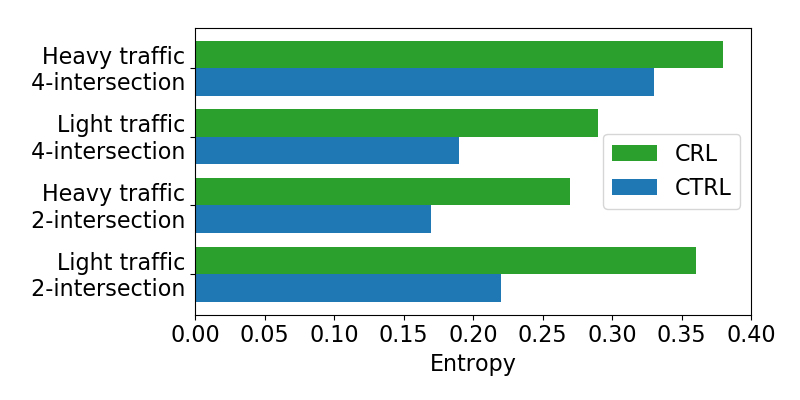
\includegraphics[width=0.45\textwidth]{figures/transfer_results_ijcai_entropy.png}
   \vspace{-2mm}
    \caption{Cycle length entropy on synthetic traffic configurations}
   \label{fig:entropy}
\end{figure}

\begin{figure}[t!]
  \centering
  \begin{tabular}{ccc}
   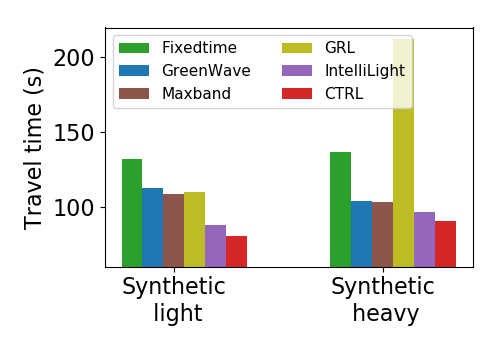
\includegraphics[width=0.225\textwidth]{figures/large_results_ijcai.png} &
   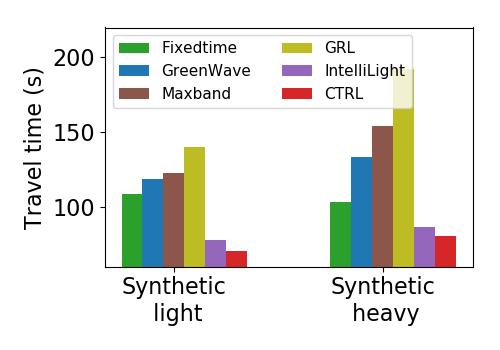
\includegraphics[width=0.225\textwidth]{figures/network_results_ijcai.png} \\
    \begin{tabular}[c]{@{}c@{}}(a) \end{tabular}&
   \begin{tabular}[c]{@{}c@{}}(b) \end{tabular}\\
   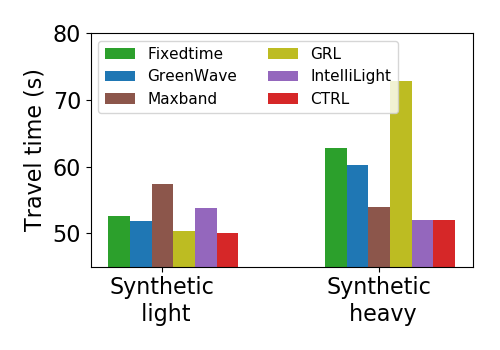
\includegraphics[width=0.225\textwidth]{figures/heter_results_ijcai.png} &
   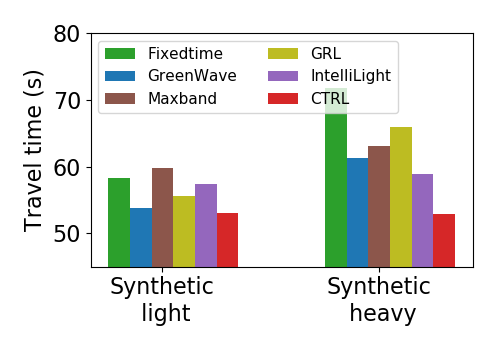
\includegraphics[width=0.225\textwidth]{figures/heter_results_leg_ijcai.png}\\
   \begin{tabular}[c]{@{}c@{}}(c)\end{tabular}&
   \begin{tabular}[c]{@{}c@{}}(d) \end{tabular}\\
   \end{tabular}
     \caption{Performance of different methods w.r.t average travel time on different road networks. (a): A 10-intersection arterial. (b): A $3\times3$ grid network.  (c) A 2-intersection arterial with different lane length. (d) A 2-intersection arterial with different number of legs.}
    \label{fig:generality}
\end{figure}


\begin{figure*}[thb]
  \centering
  \begin{tabular}{cc}
   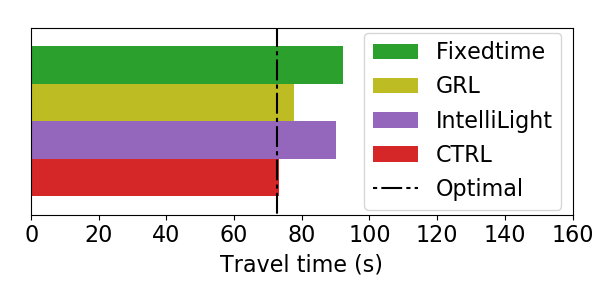
\includegraphics[width=0.42\textwidth]{figures/case_uniform_uni_ijcai.png} &
   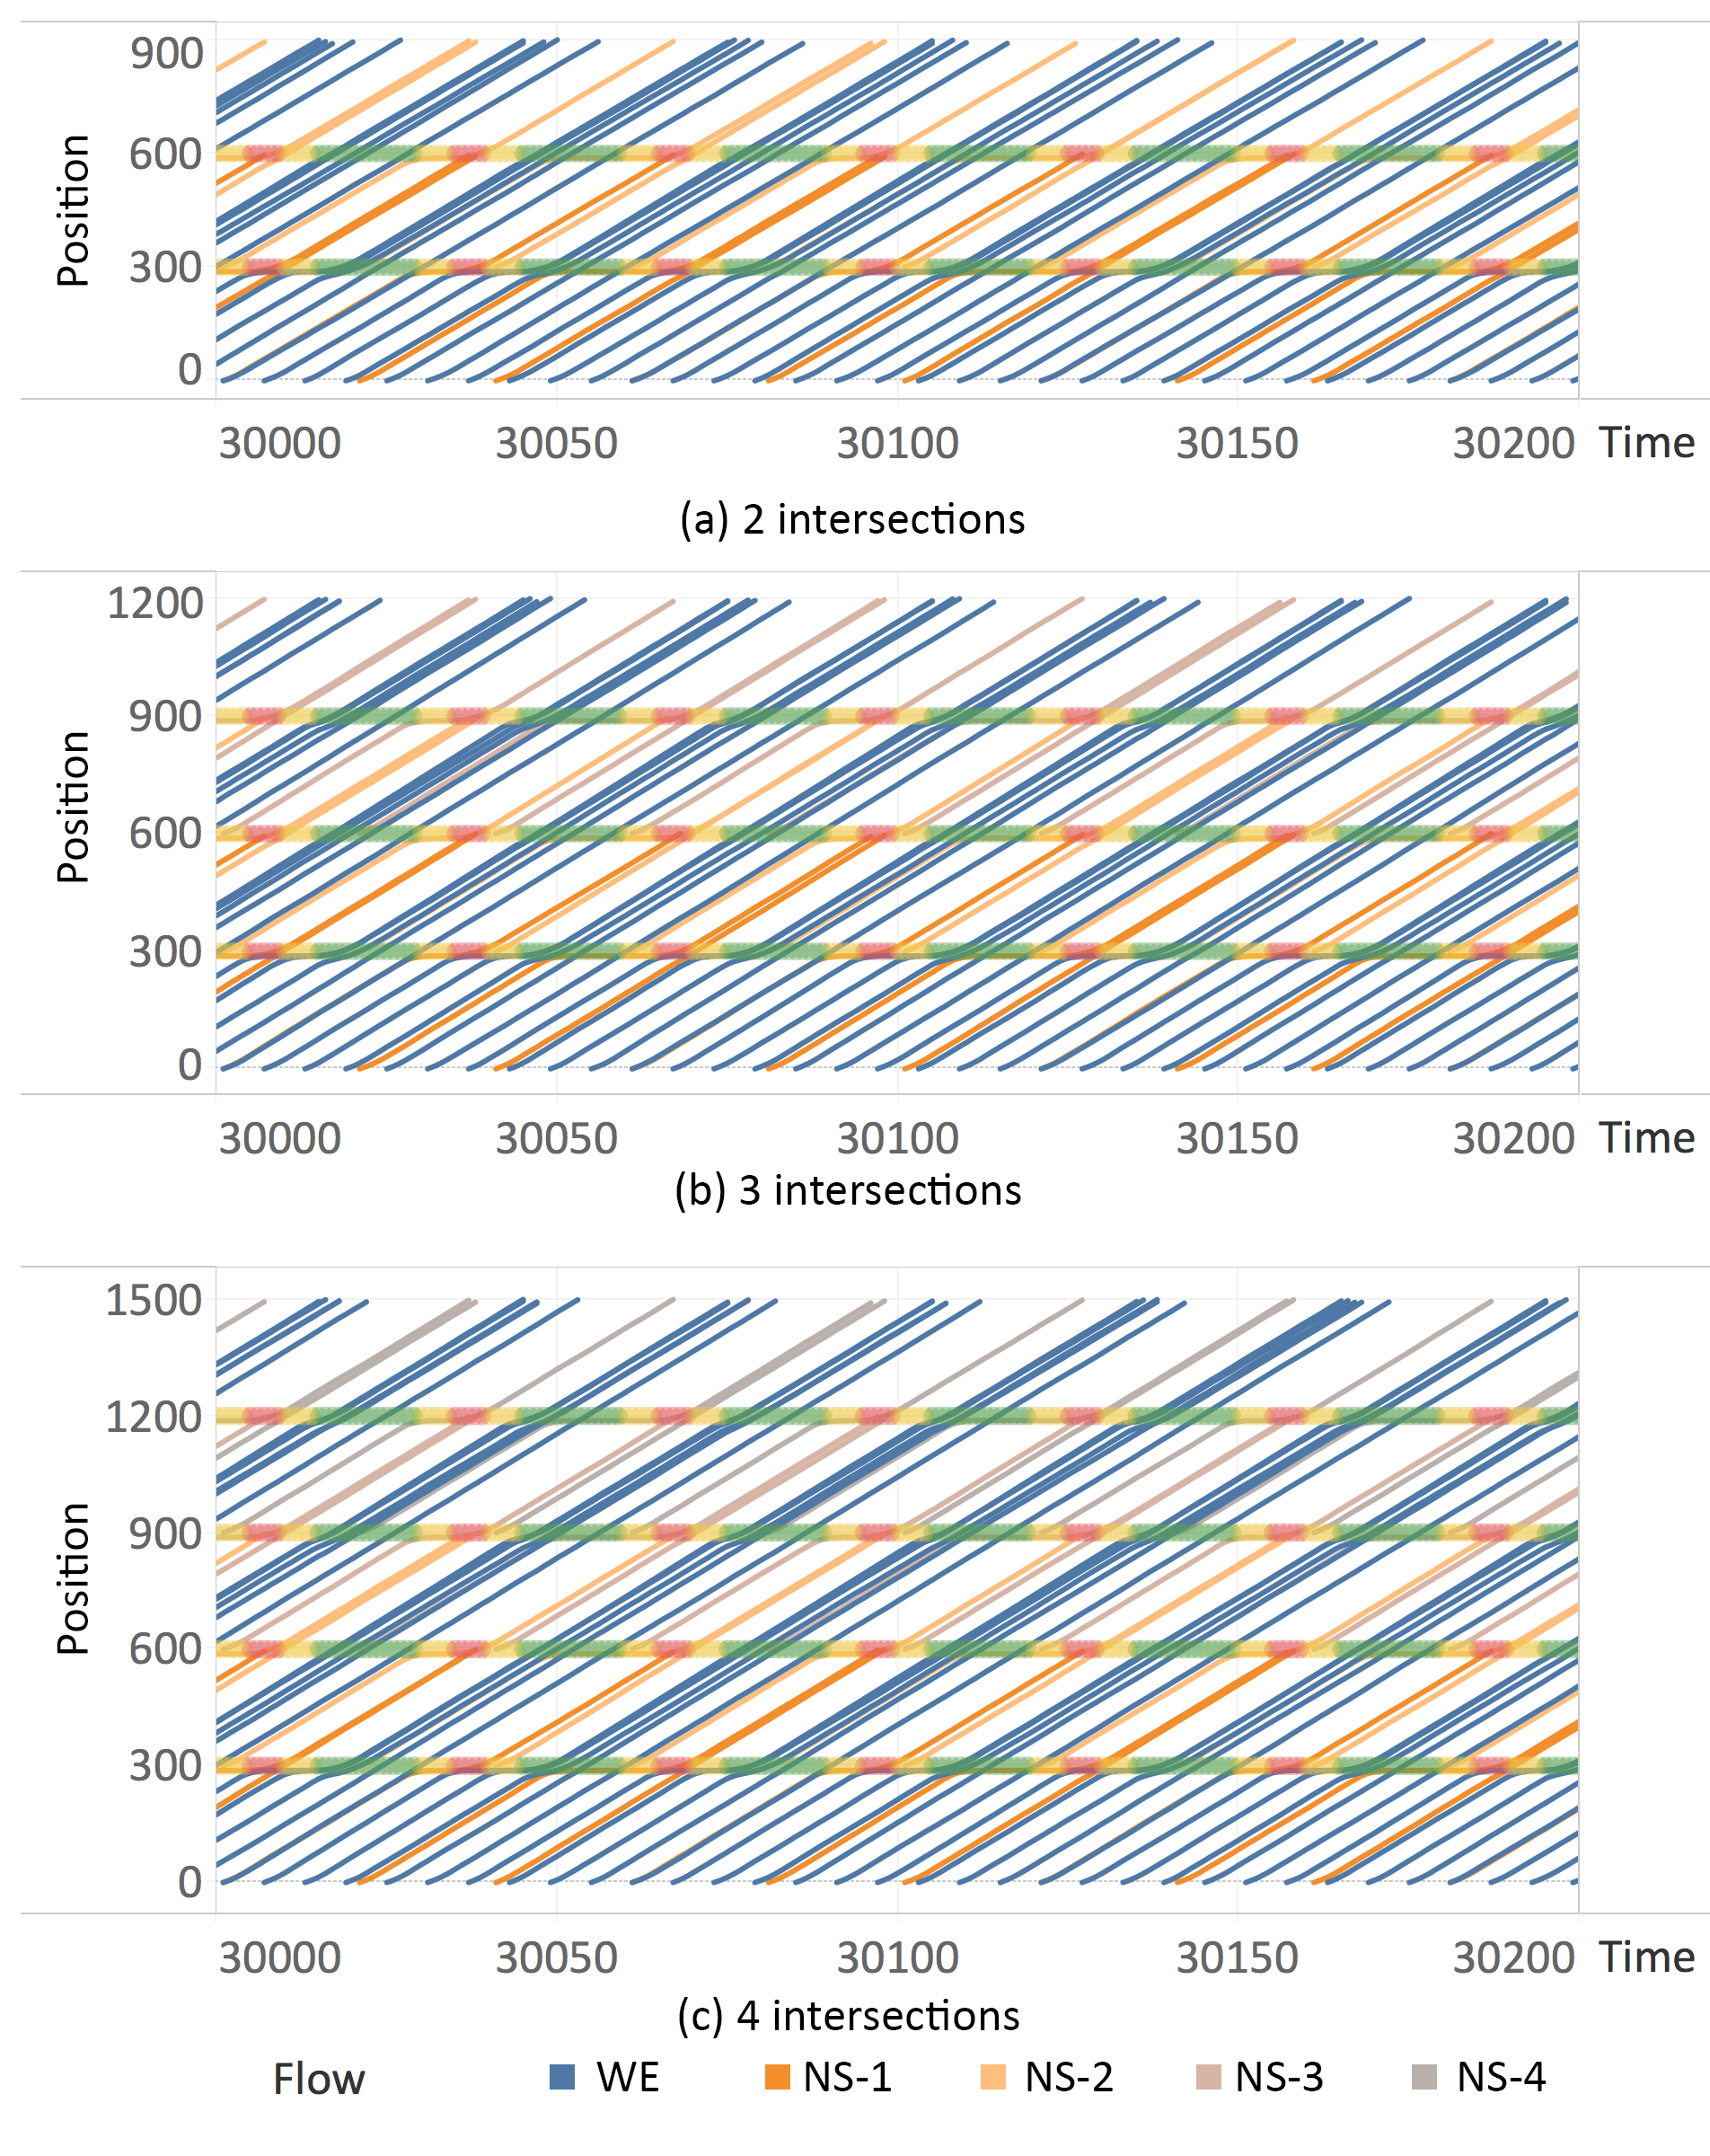
\includegraphics[width=0.45\textwidth]{figures/case_study.png} \\
   \begin{tabular}[c]{@{}c@{}}(a) Performances on uniform traffic\end{tabular}&
   \begin{tabular}[c]{@{}c@{}}(b) Policy learned by \MTDeeplight \end{tabular}\\
   \end{tabular}
     \caption{Overall performance and learned policy of proposed method under uniform one-way traffic. Left: Average travel time of all baseline methods. \Maxband is not included since it does not work under one-way traffic.  Right: Time-space diagram with signal timing plans to illustrate the green waves learned by \MTDeeplight. The green-yellow-red bands represent the change of traffic signal along the arterial. Each line in space-time diagram stands for one vehicle's trajectory.}
    \label{fig:case-study}
\end{figure*}

\subsubsection{Efficacy of transferred knowledge}
We compare a variation of our method to validate the effectiveness of transferred knowledge. In the lower part of Table~\ref{tab:overall-result}, we can see that with transferred knowledge,  \MTDeeplight consistently outperforms \MDeeplight under both synthetic and real-world traffic dataset in terms of average travel time, while the gap between them grows larger under real-world traffic.

To further investigate the efficacy of transferred knowledge, we conduct detailed experiments under synthetic traffic. We also use \textit{entropy of cycle length} to measure the steadiness of reinforcement learning agents. Under uniform traffic, a lower entropy indicates a more converged condition for reinforcement learning agents. Results in Figure~\ref{fig:entropy} show that \MTDeeplight shows a lower entropy than \MDeeplight under both light and heavy traffic situations. This is because the knowledge transferred serves as good initialization to help the model converge faster. 


% \begin{table}[tbh]
% \centering
% \caption{Cycle length entropy on synthetic traffic configurations on homogeneous and heterogeneous intersections}
% \begin{tabular}
% {p{0.05\textwidth}p{0.03\textwidth}p{0.03\textwidth}p{0.03\textwidth}p{0.03\textwidth}p{0.03\textwidth}p{0.03\textwidth}p{0.03\textwidth}p{0.03\textwidth}}
% \toprule
% Config. & 1     & 2     & 3     & 4     & 5     & 6     & 7     & 8     \\ \hline
%         & \multicolumn{8}{c}{2 homogeneous intersections}                                   \\ \hline
% \MDeeplight      & 0.28  & 0.46 & 0.22 & 1.13   & 0.36  & 1.27 & 0.27 & 1.169 \\
% \MTDeeplight & \textbf{0.16}  & \textbf{0.28} & \textbf{0.20} & \textbf{0.03} & \textbf{0.22}  & \textbf{0.08}   & \textbf{0.17} & \textbf{1.167} \\ 

% \hline
%         & \multicolumn{8}{c}{3 homogeneous intersections}                                   \\ \hline
% \MDeeplight    & 0.29  & 0.38 & 0.29 & 1.25  & 0.15  & 0.14  & 0.30 & 1.21 \\
% \MTDeeplight & \textbf{0.02} &\textbf{0.27} & \textbf{0.24} & \textbf{0.08} & \textbf{0.22}  & \textbf{1.39}   & \textbf{0.20} & \textbf{1.20} \\

% \hline
%         & \multicolumn{8}{c}{4 homogeneous intersections}                       \\ \hline
% \MDeeplight  & 0.26  & 0.52  & 0.25 & 1.19   & 0.29  & 0.10 & 0.38 & 1.208 \\
% \MTDeeplight & \textbf{0.04} & \textbf{0.29} & \textbf{0.24} & \textbf{1.14}   & \textbf{0.19} & \textbf{0.06} & \textbf{0.33} & \textbf{1.205} \\

% \hline
%         & \multicolumn{8}{c}{2 heterogeneous intersections}                                   \\ \hline
% \MDeeplight      & 1.74  & 1.16  & 1.69  & 1.58  & 1.95  & 1.99  & 1.100 & 1.30  \\
% \MTDeeplight     & \textbf{0.91}  & \textbf{0.92}  & \textbf{1.62}  & \textbf{1.26}  & \textbf{1.49}  & \textbf{1.13}  & \textbf{1.098} & \textbf{1.09} \\

% \bottomrule
% \end{tabular}
% \label{tab:entropy}
% \end{table}

\subsubsection{Generality of RL agent}
To test the generality of our RL method, we compare our method \MTDeeplight with state-of-the-art methods under following different settings:

\paragraph{Large scale arterial.} In this experiment, an arterial with 10 homogeneous intersections is utilized to test the performance of different methods on large scale arterial. As shown in Figure~\ref{fig:generality}(a), \MTDeeplight outperforms all other baselines under both light and heavy traffic.

\paragraph{Grid network.} Compared with arterials, people my also concern about the overall traffic light control for an grid network. To validate the potential of our model in the grid network, we also deploy our model on a $3\times3$ grid network. In this network, we consider the horizontal roads as arterials.
As shown in Figure~\ref{fig:generality}(b), \MTDeeplight outperforms all other baselines under both light and heavy traffic. 

\paragraph{Heterogeneous intersections.} We also employ our model to arterials with heterogeneous intersections. Specifically, two different kinds of heterogeneous intersections are investigated. One is an arterial with two heterogeneous intersection, where one intersection has 300-meter long roads and the other has 150-meter long roads. The other kind is a 2-intersection arterial where one intersection has four legs and the other has three legs. For intersections with different legs, we use zero-padding to fill in the missing values. As is shown in Figure~\ref{fig:generality}(c) and (d), our method performs consistently better than other baselines. 

\subsection{Case Study: Learning Green Wave}
As stated in Section~\ref{sec:agent-design}, our definition of state and reward is sufficient for an RL algorithm to learn the optimal policy under uniform traffic flow. Here we validate it by using the synthetic setting where conventional coordination method \Greenwave can form a green wave for traffic along the arterial and is an optimal solution as stated in ~\cite{Roess2011t}. In our experiments, the optimal offset given by \Greenwave should be approximately 30 seconds. 

\paragraph{Overall performance}
As shown in Figure~\ref{fig:case-study}(a), \MTDeeplight outperforms all the other baseline methods
and achieves almost identical performance with the optimal solution \Greenwave.

\paragraph{Learned policy.}
We further interpret the policy learned by \MTDeeplight in the form of a time-space diagram, as shown in Figure~\ref{fig:case-study}(b). 
In the time-space diagram, the trajectory of a vehicle on the arterial always move from left to right and from bottom to top. Vehicles traversing green waves will always travel at their free-flow speed. As is shown in Figure~\ref{fig:case-study}(b), the traffic signals controlled by our method can automatically form green waves along the arterial. An exemplary green wave is highlighted as the green sloped area in Figure~\ref{fig:case-study}(b). A demo of the policy learned by our agent can be found at: \url{https://bit.ly/2IQDVUv}.


% !TEX root = main.tex
\section{Conclusion}
In this paper, we propose a novel RL method for multi-intersection traffic signal control on the arterials with provable state and reward design. We also conduct experiments using both synthetic and real-world experiments and demonstrate the superior performance of our method over state-of-the-art methods. Specifically, we draw a connection between reinforcement learning with conventional transportation control methods. It is the first time there exists an RL model automatically achieving coordination along an arterial without explicit prior knowledge. 
 
 We also acknowledge the limitations of our current approach and possible future directions could be the following. We can extend the tested arterial to the network level. The authors would expect increased computational cost while introducing more agents; however, our RL model is still elegant as there is no need for further model modifications. Also, currently our model is tested on a simulation environment, thus the feedbacks of control is also simulated. A field study is needed to validate our method in the real-world environment.